\section{Kamehameha}

	\subsection{Introducción}
		El problema a resolver nos pide encontrar una posible forma de cubrir N puntos en un plano con la menor cantidad de rectas posible.
		Es decir: Minimizar la cantidad de rectas necesarias para cubrir N puntos dados.
		Notamos que encontrar un conjunto de rectas optimo que contenga al conjunto $\mathcal{P}tos$ (El conjunto de puntos dado),de que una recta queda definida univocamente dando 2(dos) puntos pertenecenecientes. El problema entonces que resolveremos sera encontrar un conjuntos de pares $\mathcal{CP}ares	    \subseteq \mathcal{P}tos \times \mathcal{P}tos$ de modo tal que las rectas inducidas por $\mathcal{CP}ares$ contengan a todo $p \in \mathcal{P}tos$ y ademas $\nexists \quad \overline{\rm \mathcal{CP}ares} / \quad \textrm{queden  inducidas rectas que contenga a todo} \quad \mathcal{P}tos$ con  $\# \overline{\rm \mathcal{CP}ares} < \# \mathcal{CP}ares$. \\
		Es este entonces el problema principal que resolveremos.\\
		Margen de notación: la recta que induce $(p,p) \in \mathcal{P}tos \times \mathcal{P}tos$ es alguna que pasa por p pero que no influye en lo otros puntos.
	
    \subsection{Desarrollo}
    	Para resolver este problema implementaremos un algoritmo de Backtracking. En el cual, el papel principal lo juega la funcion ``mejoresPares'' que es la encargada de devolver un conjunto optimo de pares que inducen las rectas que cubren todos los puntos de alguna de las maneras optimas posibles.
  		procederemos entonces a mostrar un pseudocodigo de esta funcion, (por claridad utilizaremos las funciones tradicionales de conjuntos para operar pero en realidad todos los conjuntos estan implementados sobre vectores lo que les da un caracter numerable y por lo tanto la operacion [ ]) :
  		\\ \\
  		$mejoresPares(conjunto \quad Puntos) \longmapsto conjuntoParesOptimo $\\
  		$mejoresPares(\emptyset) \equiv \emptyset$\\
  		$mejoresPares(\{ p \}) \equiv \{ (p,p) \} $\\
     	$mejoresPares(\{ p,q \}) \equiv \{ (p,q) \} $\\
     	$mejoresPares(\{ p \} \cup Ptos) :$\\
     	$Pares \gets generarConjPares(p,Ptos)$ //genero los posibles pares que pasan por p \\ \\
     	$i \gets \{0..\#Pares\}$  // genero por cada $par_i$ los mejores pares desde los LI con $par_i$
		\\
 		$\quad posiblesConvinaciones[i]=mejoresPares(sinLD(Pares[i],Ptos))$\\ 
 		\\
 		$return \gets conjMasChico(posiblesConvinaciones)$ // devuelve el conjunto de pares mas chico que tenga
		\\
		\\
		Se ve en el pseudocodigo que esencialmente lo que hacemos es generar todas las posibles rectas que pasan por punto y luego tomar la que cuando sacas los puntos que le pertenecen te quda el conjunto cuya cantidad de rectas optimas para cubrirlo sea menor. En otras palabras tomo la recta a la cual al aplicarle el algoritmo recursivamente termine teniendo la menor cantidad de pares en el conjunto que induce sus rectas.\\
		De tener el conjunto de rectas optimo solo tengo que adaptarlo con algunas operaciones $\mathcal{O}(n)$ muy sencillas para obtener la salida requerida en el ejercicio, ya que es simplemente ver quienes estan en cada recta, contarlos y asegurarme de no repetirlos si otra recta pasa por algun punto que ya tome en cuenta.
		\\ 
		\\
		En cuanto a la correctitud de la solucion, es evidente que este algoritmo funciona, osea que la convinacion de rectas es optima pues para econtrarla se la comparo con todas las posibles convinaciones de rectas que cubren a todos los posibles pares de puntos y se elegio de entre ellos el conjunto de rectas con el menor cardinal.


    \subsection{Complejidad}

    	La complejidad requerida de $\mathcal{O}(N^{N+2})$ se cumple pues, si analizamos es codigo se ve que en cada llamada recursiva se realizan operaciones de a lo sumo $\mathcal{O}(N^{2})$ ya que generar conjunto de pares que pasen por un punto es $\mathcal{O}(N)$ (el punto en cuestion juntarlo con los n-1 restantes), generar un conjunto sin Linearmente dependientes con un punto tambien es $\mathcal{O}(N)$ (pues es chequear una igualdad en  $\mathcal{O}(1)$ para cada punto) y esto se ejecuta a lo sumo N veces lo que no supera entonces la complejidad $\mathcal{O}(N^{2})$ y realizar buscar un minimo sobre un vector de n elementos es tambien $\mathcal{O}(N)$. \\
		Por otro lado si vemos la cantidad de llamadas recursivas que se realizan, el esquema seria:\\
		En la primer iteracion se generan N llamadas recursivas una para cada par considerado.\\
		-En el segundo nivel de llamada cada una de las N llamadas genera n-2 llamadas (pues trabajan sobre un conjunto de puntos al que le falta un par). \\ 
		Continua asi entonces en cada nivel llamando a menos llamadas hasta llegar a los casos base.
		Si bien basado en el esquema planteado se observa que podriamos acotar la complejidad del algorimo por un tiempo factorial si hilaramos fino. De manera mas sencilla aun se ve que se puede acotar la cantidad de llamadas recursivas por $N^{N}$ dando una complejidad de la funcion ``mejoresPares'' de a lo sumo $\mathcal{O}(N^{N+2})$ pues es la multiplicacion de la cantidad de llamadas por el lo que tarda cada una.Y como el resto del codigo no utiliza funcion con niguna complejidad relevante (no pasa el $\mathcal{O}(N^{2})$ la parte no recursiva) entonces podemos concluir que el algoritmo $ \in \mathcal{O}(N^{N+2})$.


    \subsection{Código}


    \subsection{Experimentación}

    	\subsubsection*{Experimento 1}\;

    		En este experimento se analizará la variación del tiempo de ejecución del algoritmo cuando varía la cantidad de guerreros enemigos. Para ello se generarán diferentes archivos con las coordenadas de los enemigos, uno por cada tamaño de bando contrario. Las coordenadas de los soldados serán aleatorias tomando una cota como máximo valor posible para las variables x e y. Luego pasando esos archivos como parámetro de entrada al problema de kamehameha, se medirán los tiempos de ejecución. \;

    	\subsubsection*{Datos de entrada}\;
    		Los tamaños del bando enemigo tomados fueron $5$ $7$ $9$ $10$ $11$ $12$ $13$ $14$ $15$ $16$ $17$ $18$.
			Para generarlos se utilizó el generador.cpp que se encuentra en la carpeta exp/kamehameha/exp1 y para correrlo se utilizó el exp1.sh que se encuentra en la misma carpeta. \;
			Con el fin de acercarse a los valores reales y descartar posibles falsos resultados, se ejecuta la resolución del problema para cada uno de los tamaños de equipo siete veces y se calcula el promedio de los tiempos medidos.\;

      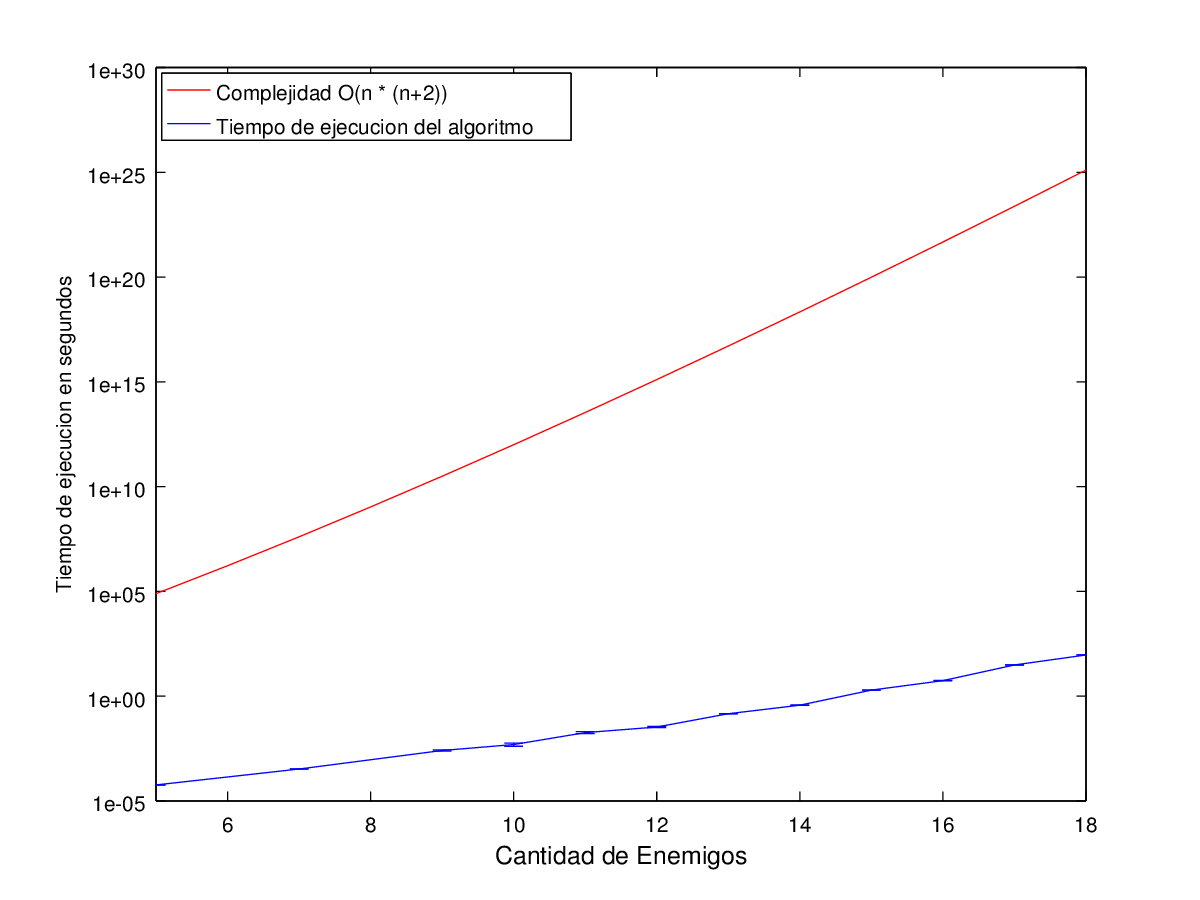
\includegraphics[height=11cm]{graficos/kamehameha-exp1.png}



		\subsubsection*{Conclusiones}\;

			Como se puede observar en el gráfico, el tiempo de ejecución aumenta de manera exponencial con respecto a la cantidad de guerreros enemigos dando una complejidad de $\mathcal{O}(N^{N+2})$. Esto es así ya que el algoritmo busca todas las posibles combinaciones de disparos a efectuar y de todas ellas elige la que requiera menor cantidad de lanzamientos. \;

		\;
		\;
		
    	\subsubsection*{Experimento 2}\;
    		En este experimento vamos a comparar como varia el tiempo de ejecución del algoritmo para casos bordes. En el primero tomaremos guerreros que se encuentren dispuestos de forma alineada de manera que con un solo disparo se pueda matar a todo el equipo enemigo. En el segundo, los guerreros estarán distribuidos de forma tal que solo se pueda matar de a dos de ellos con un disparo. Tomaremos la misma cantidad de soldados del bando enemigo para ambos casos. \;

    	\subsubsection*{Datos de entrada}\;
    		El tamaño del bando enemigo utilizado fue de 18 guerreros.
			Para generar el primer caso se utilizó el generador.cpp y para el segundo el generador2.cpp que se encuentran en la carpeta exp/kamehameha/exp2. Para correrlos se utilizó el exp2.sh que se encuentra en la misma carpeta.\;
			Con el fin de acercarse a los valores reales y descartar posibles falsos resultados, se ejecuta la resolución del problema para cada uno de los tamaños de equipo siete veces y se calcula el promedio de los tiempos medidos.\;

      	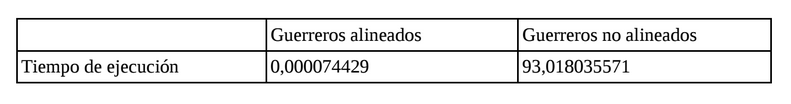
\includegraphics[height=2cm]{graficos/tabla.png}


		\subsubsection*{Conclusiones}\;
			Como se puede ver en la tabla, el tiempo de ejecución cuando los puntos se encuentran alineados es mucho menos que cuando solo puedo matar de a dos guerreros enemigos. Esto se debe a que el algoritmo toma todos los posibles pares de guerreros y para cada uno de ellos se fija como armar mas pares sin tener en cuenta los soldados que quedan alineados con la recta que une al primer par. En el caso que estén todos alineados la complejidad bajará a $\mathcal{O}(N)$ ya que para ningún posible par que se pueda armar en un primer momento quedan mas guerreros que no se encuentren alineados con el primer par. Por lo que solo tomará posibles pares de guerreros y finalizará la ejecución. En cambio cuando están muy desalineados, por cada par inicial quedan exactamente $n - 2$ guerreros para reordenar en pares, generando así una complejidad de $\mathcal{O}(N^{N+2})$.


